\documentclass{beamer}
\usepackage[latin1]{inputenc}
\usepackage{tikz}
\usetheme{Warsaw}
\title[Crono]{Crono \\ A new programming language of sorts}
\author{Brad Burlage \\ James Debo \\ Joey Mangieri}
\begin{document}

\begin{frame}
\titlepage
\end{frame}


\begin{frame}{Grammar}
$Program \rightarrow (List\ |\ Atom)*$ \\
$List \rightarrow (\ (List\ |\ Atom)*\ )$ \\
$Atom \rightarrow Nil\ |\ Integer\ |\ Symbol$ \\
$Nil \rightarrow \text{``nil'' } |\ ()$ \\
\end{frame}
\begin{frame}{Types}
\tikzstyle{state} = [rectangle, node distance=6em]
\begin{tikzpicture}
  \node [state, name=ct]   {CronoType};
  \node [state, name=atom, below of=ct, left of=ct] {Atom};
  \node [state, name=cons, below of=ct, right of=ct] {Cons};
  \node [state, name=func, below of=atom, left of=atom] {Function};
  \node [state, name=cf, below of=func, left of=func]   {CronoFunction};
  \node [state, name=lf, below of=func, right of=func]   {LambdaFunction};
  \node [state, name=sym, below of=atom, right of=atom]  {Symbol};
  \node [state, name=num, below of=atom]  {CronoNumber};
  \node [state, name=nil, below of=cons]  {Nil};

  \draw (ct.south) edge (atom.north);
  \draw (ct.south) edge (cons.north);
  \draw (cons.south) edge (nil.north);
  \draw (atom.south) edge (nil.north);
  \draw (atom.south) edge (func.north);
  \draw (atom.south) edge (num.north);
  \draw (atom.south) edge (sym.north);
  \draw (func.south) edge (cf.north);
  \draw (func.south) edge (lf.north);
\end{tikzpicture}
\end{frame}
\begin{frame}{Interpreter}
\begin{center}
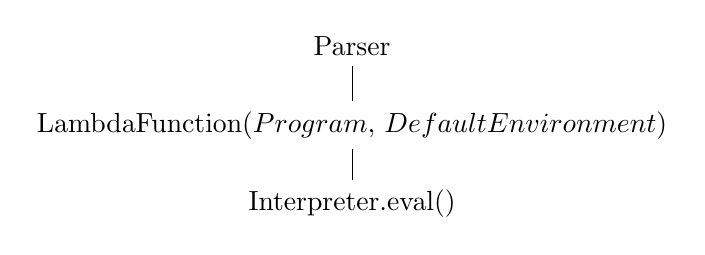
\begin{tikzpicture}
  \node [name=parser] {Parser};
  \node [name=lf, below of=parser] {LambdaFunction($Program$, $DefaultEnvironment$)};
  \node [name=interp, below of=lf] {Interpreter.eval()};

  \draw (parser.south) edge (lf);
  \draw (lf.south) edge (interp);
\end{tikzpicture}
\end{center}
\end{frame}
\begin{frame}{Interpreter}
\begin{center}
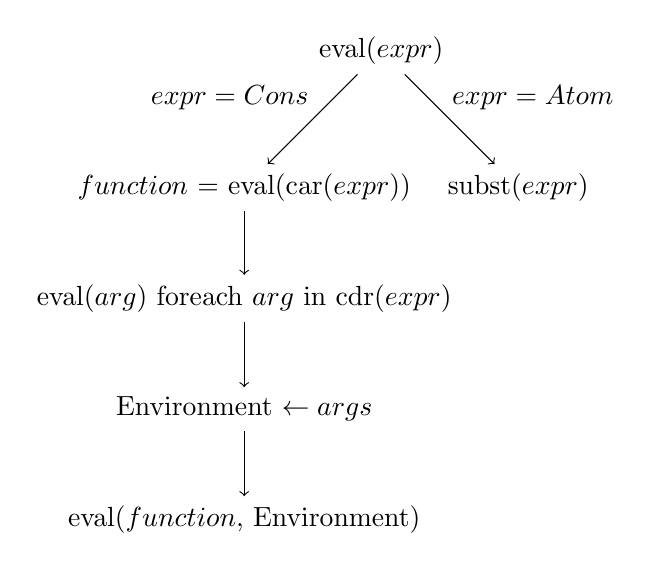
\begin{tikzpicture}
  [ ->, above, node distance=4em]
  \node [name=eval, node distance=6em] {eval($expr$)};
  \node [name=atom, below right of=eval, node distance=7em] {subst($expr$)};
  \node [name=cons, below left of=eval, node distance=7em] {$function$ = eval(car($expr$))};
  \node [name=cons2, below of=cons] {eval($arg$) foreach $arg$ in cdr($expr$)};
  \node [name=cons3, below of=cons2] {Environment $\leftarrow args$};
  \node [name=cons4, below of=cons3] {eval($function$, Environment)};

  \path (eval) edge node {$\qquad\qquad\qquad expr = Atom$} (atom)
        (eval) edge node {$expr = Cons\qquad\qquad\qquad$} (cons)
        (cons) edge (cons2)
        (cons2) edge (cons3)
        (cons3) edge (cons4);
\end{tikzpicture}
\end{center}
\end{frame}
\begin{frame}{Environment \& CronoFunctions}
\begin{center}
Environment = \{$Symbol$ : $CronoType$\} \\
\hfill \\
\hfill \\
\hfill \\
\begin{tabular}{l l l l l l}
Default environment = & \{ \\
&&quote,& let,& if, \\
&&cons,& car,& cdr, \\
&&define,& lambda, \\
&&add,& subtract,& multiply,& divide, \\
&&==,& $>$,& $<$, \\
&&set,& load,& print \\
&\} \\
\end{tabular}
\end{center}
\end{frame}
\begin{frame}{CronoOptions}
\begin{itemize}
\item Parser and interpreter debug output
\item Show/hide atom evaluation
\item Show environment during execution
\item Use static or dynamic scoping
\item Show types in the environment
\item Show closures
\end{itemize}
\end{frame}
\begin{frame}{TODO}
\begin{itemize}
\item Strings
\item Haskell-like type checking
\item Setting CronoOptions via POSIX command line flags
\item Improve and possibly expand CronoOptions
\item Extend CronoNumber
\item Better error handling
\end{itemize}
\end{frame}

\end{document}
